\documentclass{article}

\title{Regularization techniques for Deep Learning}
\author{Vladimir Feinberg}

\usepackage{nicefrac}
\usepackage[hidelinks]{hyperref}
\usepackage{xcolor}
\usepackage{url}
\usepackage{lmodern}
\usepackage{amsmath}
\usepackage{amsthm}
\usepackage{amssymb}
\usepackage{amsfonts}
\usepackage{enumerate}
\usepackage{graphicx}
\usepackage{fullpage}
\usepackage{bbm}
\usepackage{caption}
\usepackage{mathrsfs}
\usepackage[all]{xy}

\newcommand{\pa}[1]{ \left({#1}\right) }

\def \N {\mathbb{N}}
\def \Nbr {\mathcal{N}}
\def \Q {\mathbb{Q}}
\def \F {\mathbb{F}}
\def \then {\implies &}
\def \oif {\Longleftrightarrow &\,}
\def \given {\text{Given }&}
\def \assume {\text{Assume }&}
\def \thfr {\therefore &\enskip}
\def \bij {\leftrightarrow}
\def \inj {\rightarrowtail}
\def \sur {\twoheadedrightarrow}
\def \Z {\mathbb{Z}}
\def \R {\mathbb{R}}
\def \C {\mathbb{C}}
\def \T {\mathbb{T}}
\def \iff {\Longleftrightarrow}
\def \kron {\boldsymbol\delta}
\def \indicator {\mathbbm{1}}

\def\Ta{\textbf{a}}
\def\Tm{\textbf{m}}
\def\Tb{\textbf{b}}
\def\Tc{\textbf{c}}
\def\Td{\textbf{d}}
\def\Te{\textbf{e}}
\def\Tv{\textbf{v}}
\def\Tx{\textbf{x}}
\def\Tw{\textbf{w}}
\def\Ty{\textbf{y}}
\def\Tk{\textbf{k}}
\def\Tt{\textbf{t}}
\def\Tz{\textbf{z}}
\def\Tl{\textbf{l}}
\def\quotient{\mathclose{}/\mathopen{}}
\def\Tf{\textbf{f}}
\def\Th{\textbf{h}}
\def\Tg{\textbf{g}}
\def\sumn{\sum_{n=0}^\infty}
\def\limn{\lim_{n\rightarrow\infty}}
\def\prodn{\prod_{n=0}^\infty}

\def\bsz{\textbf{0}}
\def\bs1{\textbf{1}}
\def\bsa{{\boldsymbol\alpha}}
\def\bse{{\boldsymbol\eta}}
\def \bss{ {\boldsymbol\sigma}}
\def \bsth{ {\boldsymbol\theta}}

\DeclareMathOperator{\conv}{conv}
\DeclareMathOperator\cat{cat}
\DeclareMathOperator\adj{adj}
\DeclareMathOperator{\Laplace}{Laplace}
\DeclareMathOperator\Poisson{Poisson}
\DeclareMathOperator\Id{Id}
\DeclareMathOperator\Uniform{Uniform}
\DeclareMathOperator\mathProb{\mathbb{P}}
\def\P{\mathProb} % need to overwrite stupid paragraph symbol
\DeclareMathOperator\mathExp{\mathbb{E}}
\def \E {\mathExp}


\newcommand{\stc}[1]{\widetilde{#1}}   
\newcommand{\set}[2]{ \left\{ #1 \,\middle|\, #2 \right\} }
\newcommand{\idx}[3]{ \left\{ #1 \right\}_{ #2 }^{ #3 } }
\newcommand{\card}[1]{\left\vert{#1}\right\vert}
\newcommand{\colv}[1]{\begin{pmatrix} #1 \end{pmatrix}}
\newcommand{\mat}[1]{\begin{pmatrix} #1 \end{pmatrix}}
\newcommand{\detmat}[1]{\begin{vmatrix} #1 \end{vmatrix}}
\newcommand{\spanb}[1]{\text{span}\{ #1 \}}
\newcommand{\abs}[1]{\left|#1\right|}
\newcommand{\opcat}[1]{#1^{\text{op}}}
\newcommand{\Inner}[1]{\left\langle #1 \right\rangle}
\newcommand{\Innercpy}[1]{\Inner{ #1, #1 }}
\newcommand{\norm}[1]{\left\| #1 \right\|}% use instead of $\|x\|$

\def\eqd{\mathrel{\overset{\Delta}{=}}}

\DeclareMathOperator{\diag}{diag}
\DeclareMathOperator{\vcdim}{VC-dim}
\DeclareMathOperator*{\Err}{\text{err}}
\DeclareMathOperator*{\ErrE}{\mathbb{E}}
\DeclareMathOperator{\Tr}{tr}
\DeclareMathOperator{\Dim}{dim}
\DeclareMathOperator{\Rank}{rank}
\DeclareMathOperator*{\argmin}{argmin}
\DeclareMathOperator*{\proj}{proj}
\DeclareMathOperator{\Ker}{ker}
\DeclareMathOperator{\Diam}{diam}
\DeclareMathOperator{\Int}{int}
\DeclareMathOperator{\Clo}{clo}
\DeclareMathOperator{\sgn}{sgn}
\DeclareMathOperator{\MyRe}{Re}
\DeclareMathOperator{\MyIm}{Im}
\DeclareMathOperator{\image}{image}
\DeclareMathOperator{\colim}{colim}
\DeclareMathOperator{\Supp}{supp}
\DeclareMathOperator{\Var}{var}
\DeclareMathOperator{\Hom}{hom}
\DeclareMathOperator{\Ob}{ob}
\DeclareMathOperator{\El}{el}
\DeclareMathOperator\power{{\mathcal{P}}}
\DeclareMathOperator{\Nat}{Nat}
\DeclareMathOperator{\cone}{cone}
\DeclareMathOperator{\vectorize}{vec}
\DeclareMathOperator{\matricize}{mat}

% probability stuff
\def \sa {{$\sigma$-algebra}}
\def\OR{{\overline{\R}}}
\def\OX{{\overline{X}}}

\def\mcU{{\mathcal{U}}}
\def \mcX {\mathcal{X}}
\def \mcS {\mathcal{S}}
\def \mcY {\mathcal{Y}}
\def \mcH {\mathcal{H}}
\def \mcD {\mathcal{D}}
\def \mcC {\mathcal{C}}
\def \mcA {\mathcal{A}}
\def \mcK {\mathcal{K}}
\def \mcM {\mathcal{M}}
\def\mcG{{\mathcal{G}}}
\def\mcH{{\mathcal{H}}}
\def\mcF{{\mathcal{F}}}
\def\mcB{{\mathcal{B}}}
\def\mcE{{\mathcal{E}}}
\def\mcI{{\mathcal{I}}}
\def\mcQ{{\mathcal{Q}}}
\def\mcM{{\mathcal{M}}}
\def\mcC{{\mathcal{C}}}
\def\mcT{{\mathcal{T}}}
\def\mcO{{\mathcal{O}}}
\def\mcJ{{\mathcal{J}}}

\makeatletter
\DeclareFontFamily{U}  {MnSymbolF}{}
\DeclareSymbolFont{symbolsMN}{U}{MnSymbolF}{m}{n}
\SetSymbolFont{symbolsMN}{bold}{U}{MnSymbolF}{b}{n}
\DeclareFontShape{U}{MnSymbolF}{m}{n}{
    <-6>  MnSymbolF5
   <6-7>  MnSymbolF6
   <7-8>  MnSymbolF7
   <8-9>  MnSymbolF8
   <9-10> MnSymbolF9
  <10-12> MnSymbolF10
  <12->   MnSymbolF12}{}
\DeclareFontShape{U}{MnSymbolF}{b}{n}{
    <-6>  MnSymbolF-Bold5
   <6-7>  MnSymbolF-Bold6
   <7-8>  MnSymbolF-Bold7
   <8-9>  MnSymbolF-Bold8
   <9-10> MnSymbolF-Bold9
  <10-12> MnSymbolF-Bold10
  <12->   MnSymbolF-Bold12}{}
\DeclareMathSymbol{\tbigtimes}{\mathop}{symbolsMN}{2}
\newcommand*{\bigtimes}{%
  \DOTSB
  \tbigtimes
  \slimits@ 
}
\makeatother

% category theory arguments
% more equality: http://tex.stackexchange.com/questions/333629/
\newcommand\superequiv{ \mathrel{\rlap{\raisebox{\fontdimen22\textfont2}{$ = $}}\raisebox{-0.5\fontdimen22\textfont2}{$ = $}}}
\newcommand{\catfst}{{-}}
\newcommand{\catsnd}{{=}}
\newcommand{\cattrd}{{\equiv}}
\newcommand{\catfth}{{\superequiv}}


\newcommand{\nurl}[2]{\href{ #1 }{\color{blue}\underline{#2}}}

\begin{document}

\maketitle

\section{Regularization}

Regularization shrinks the capacity of an ANN. In other words, it restricts the richness of the family of functions which the ANN can take the value of. As Vincent Vanhouke puts it in his \nurl{https://www.udacity.com/course/deep-learning--ud730}{Udacity course}, ANN regularization can be likened to fitting into tight jeans, where extremely expressive model classes are tightened by generic regularization techniques, which seem to find a ``right fit'' in many problems, empirically speaking.

At a high level, regularization changes the objective from usual loss $J(\vtheta)$ to loss plus weight penalty $J(\vtheta)+\Omega(\vtheta)$ or loss plus constraints. In both supervised and unsupervised models this has justification in moving overfit models of high capacity to those of appropriate capacity for the problem: lower variance for a bit higher bias, where the bias and variance are with respect to the loss $J$ on the training set as an estimator for the loss on the entire data distribution.

In the sections that follow, we recount general regularization techniques for ANNs, most of which were collected from Dr. Goodfellow's \nurl{http://www.deeplearningbook.org/contents/mlp.html}{Deep Learning Book}.

\section{Weight Decay}

For all affine transforms let the weight matrix terms (not bias), vectorized, be $\vw$. Add $\Omega(\vtheta)=\frac{\alpha}{2}\norm{\vw}_2^2$. Intuitively, bias is unrestricted because it only interacts with one variable directly (the output feature map), so it isn't prone to overfitting. For a quadratic approximation of the loss at $J(\vtheta)$, with hessian $H=Q\Lambda Q^\top$, $L^2$ regularization would result in a new optimum $Q(\Lambda+\alpha I)^{-1}\Lambda Q^\top \vw_*$ where $\vw_*$ is the unconstrained optimum. If $\vv_i$ is the $i$-th eigenvector of $H$ and $\lambda_i$ its eigenvalue, then the regularization adjusts the solution by rescaling the $\vv_i$-th component of $\vw_*$ by a factor of $\frac{\lambda_i}{\lambda_i+\alpha}$. Regularization can also be viewed as constraints by identifying that $\alpha$ is a KKT multiplier: a fixed $\alpha$ corresponds to optimizing $\min J(\vtheta)$ such that $\norm{\vw}\le k$ for some $k$, which is in practice difficult to find given $\alpha$ (Fig.~\ref{fig:reg}). $L^2$ regularization is equivalent to Bayesian MAP if weights have $N(0,\alpha^{-1})$ prior.
\begin{figure}[!h]
\centering
{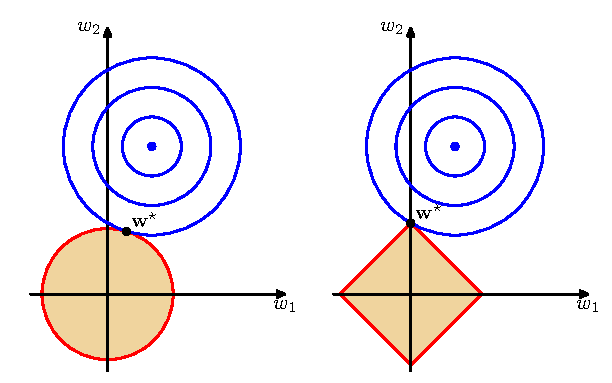
\includegraphics[width=0.75\textwidth]{reg.pdf}}
  \caption{Regularization as constrained optimization: the above shows the contour plots of a quadratic objective, and $L^2,L^1$ regularizations, respectively, as constraints constructed by weighing the objective against the shape of the regularizer's ball. Image from Bishop's Pattern Recognition and Machine Learning, Chapter 3, page 146.}
\label{fig:reg}
\end{figure}

\textbf{Proximal Regularization}. Similar to weight decay, but $\Omega(\vtheta)=\alpha\norm{\vw}_1$. Assuming a (convex) diagonal Hessian approximation to $J(\vtheta)$ (more strict than above), the $i$-th component solution is pulled down to
$$w_i=\begin{cases}
\pa{\abs{w_i}-\frac{\alpha}{H_{i,i}}}\sgn w_i  & H_{i,i}>0, \abs{w_i}>\frac{\alpha}{H_{i,i}}\\
  0 & \text{otherwise}
\end{cases}$$
$L^1$ regularization is equivalent to Bayesian MAP if weights have $\Laplace(0, \alpha^{-1})$ prior.

\textbf{Early Stopping}. Stop training if validation increases; even if training is unconverged. If validation set is large, you miss out on a lot of data. More complicated algorithms are necessary to find an applicable early stopping time when re-training to include validation set (see \nurl{http://www.deeplearningbook.org/contents/regularization.html}{Dr. Goodfellow's DL book}, Algorithm 7.3). Early stopping is similar to $L^2$ regularization, and for quadratic loss it is just that (Fig.~\ref{fig:earlystop}).
\begin{figure}[!h]
\centering
{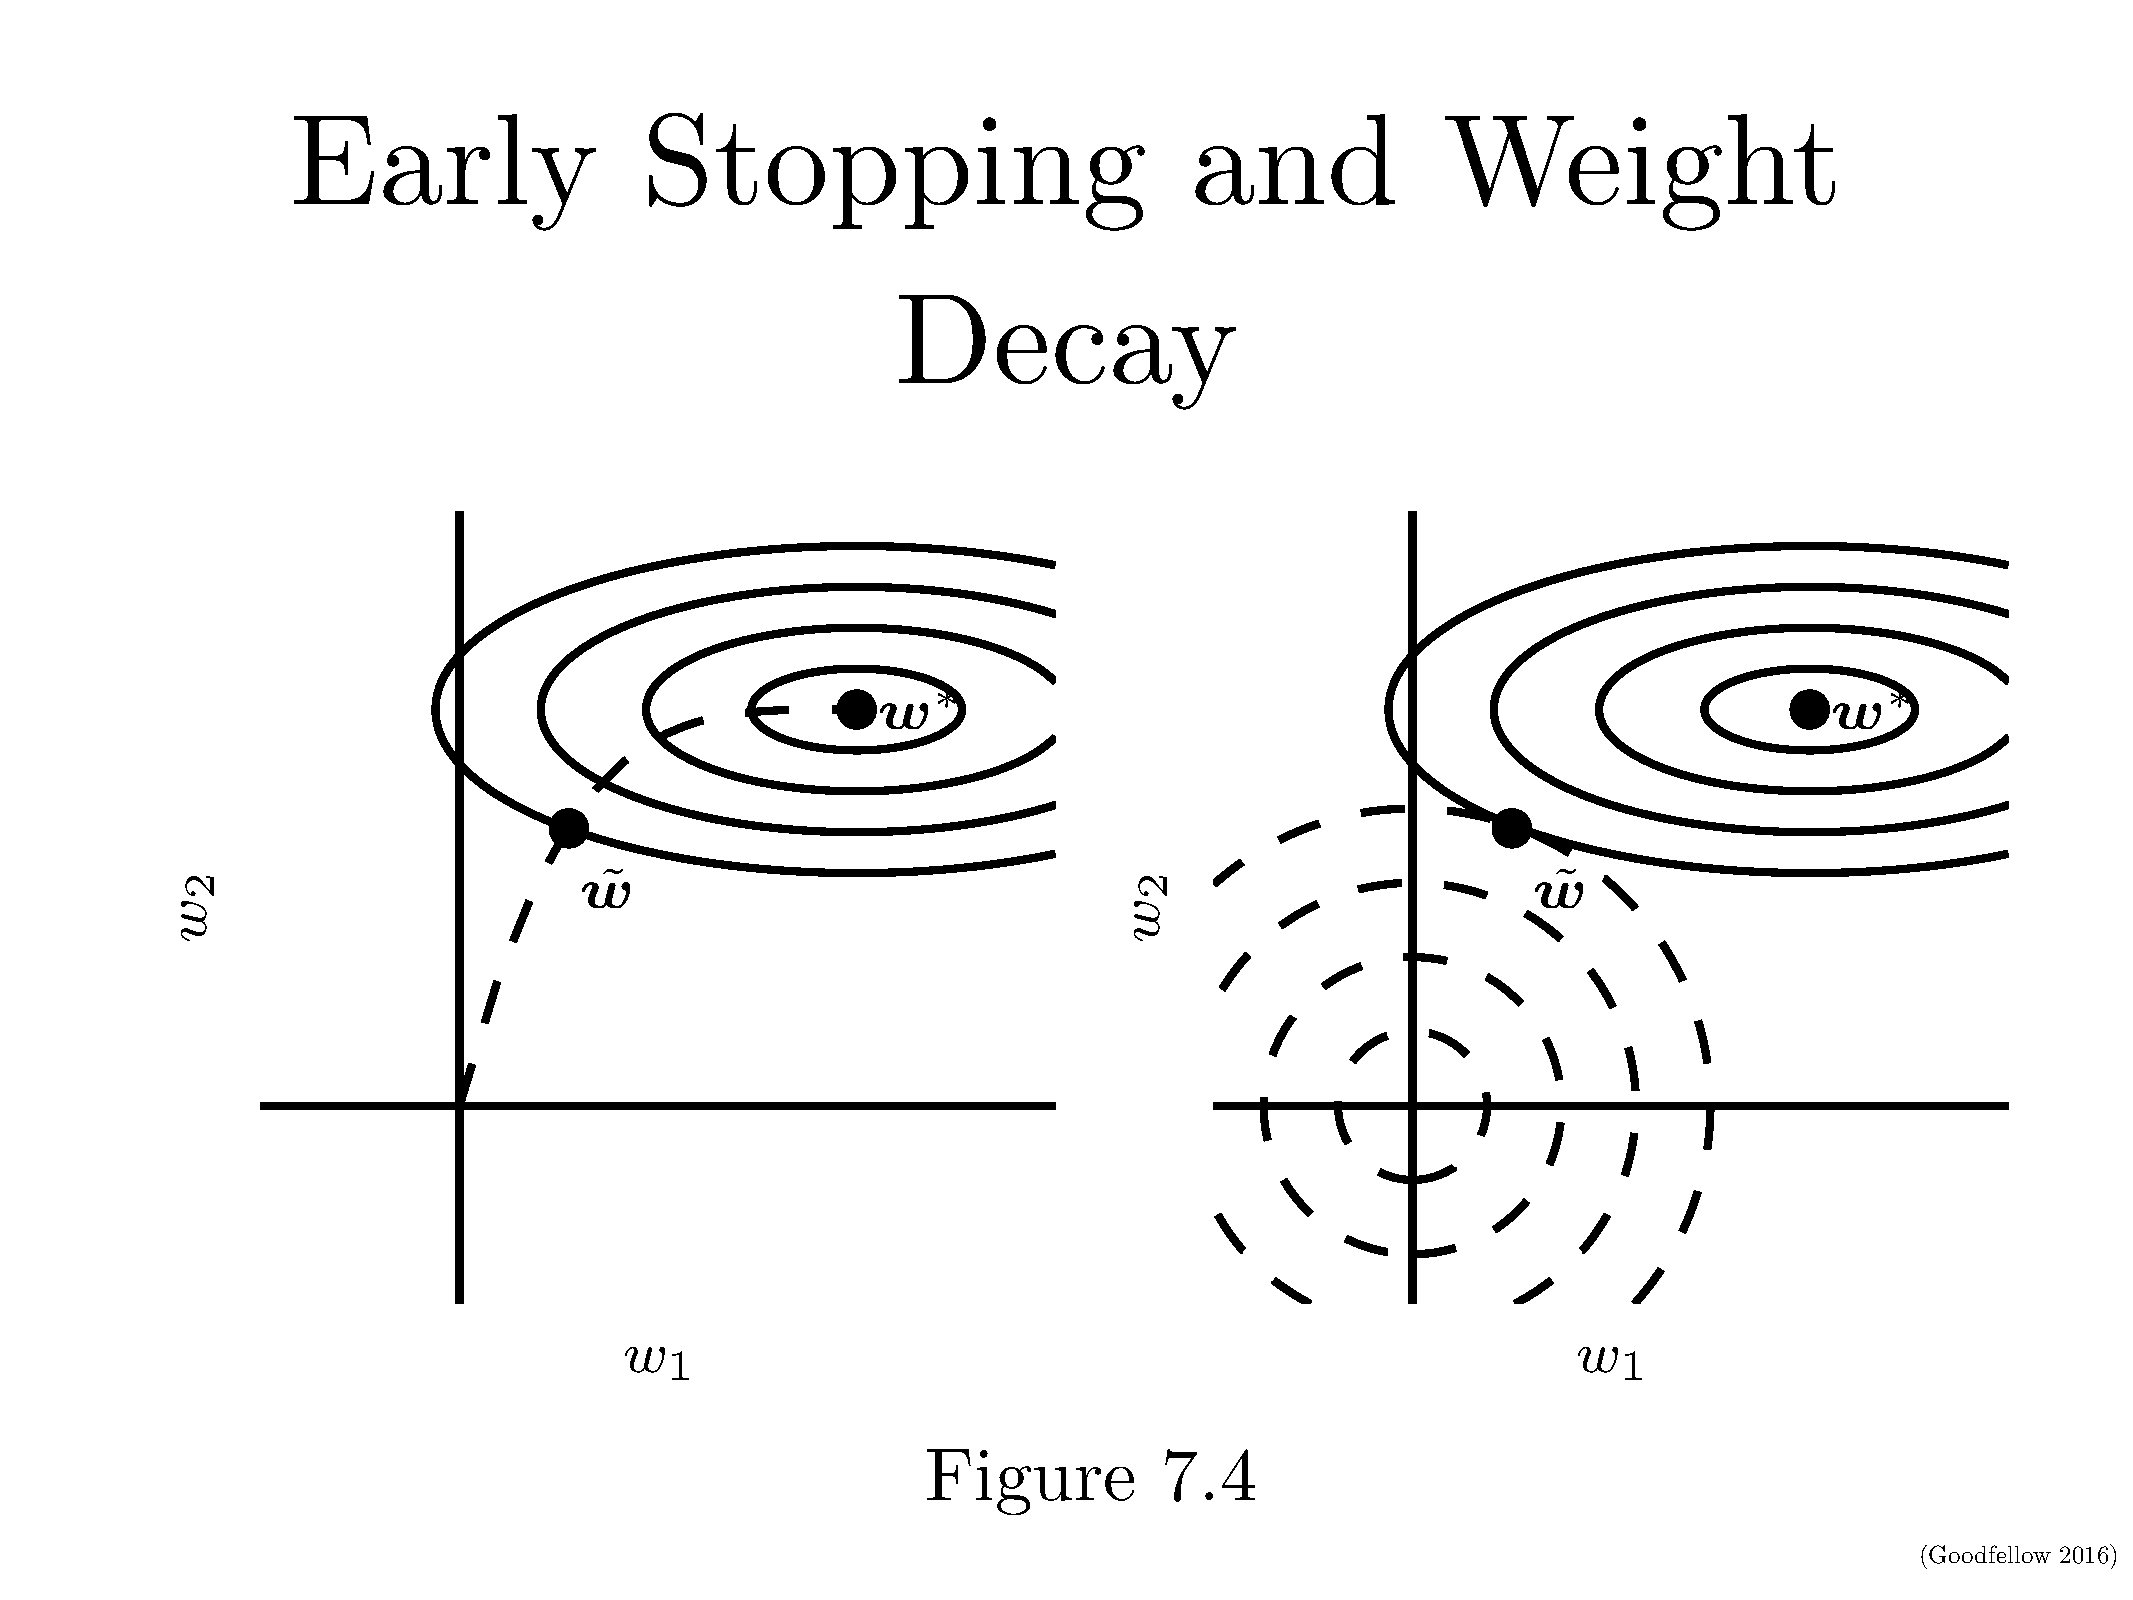
\includegraphics[width=0.75\textwidth]{early-stop.pdf}}
  \caption{From Dr. Goodfellow's DL book lecture, Chapter 7.}
\label{fig:earlystop}
\end{figure}

Early stopping can thus be viewed as an efficient way of regularizing weights just the right amount for the problem at hand, whereas we might have to cross-validate multiple settings of $\alpha$ to find an appropriate value for the $\alpha$ hyperparameter. Nonetheless, early stopping still suffers from generalization issues of overfitting to the validation set, see discussions in \nurl{http://www.tandfonline.com/doi/abs/10.1080/00207179508921605}{Sjöberg and Ljung 1995} and \nurl{http://www.mitpressjournals.org/doi/abs/10.1162/089976699300016557}{Cataltepe et al 1999}.

\section{Dataset Augmentation and Manifold Learning}

Modify supervised pairs $(\vx, y)$ to include $(T(\vx), y)$ where $T$ is a transformation we expect the classifier to be invariant to. Noise injection into inputs, too can be a form of dataset augmentation. An automatic technique for doing this is tangent propagation (\nurl{https://papers.nips.cc/paper/4409-the-manifold-tangent-classifier}{Rifai et al 2011}), which adds a penalty if the output is sensitive to changes along learned manifold vectors $\vv_i$: $\Omega(f)=\sum_i\pa{\vv_i^\top\nabla f)^2}$.

\section{Noise Robustness}

(\nurl{https://papers.nips.cc/paper/4329-practical-variational-inference-for-neural-networks}{Graves 2011}). Inject noise into weights during training, forcing learned weights to be robust to small variations.

\section{Parameter Sharing}

Reuse part of a network for another task, encoding prior knowledge that the feature maps must be the same between two tasks. CNNs, discussed in a separate document (\nurl{https://github.com/vlad17/ml-notes/tree/master/deep-learning}{root}), are a form of parameter sharing, since the linear matrix $W$ is restricted to a convolution transform.

\section{Ensemble Methods}

Bagging uses votes of several models: $k$ uncorrelated models will tend to have $\nicefrac{1}{k}$-th generalization error when bagged. Training data can be resampled to create more uncorrelated models.

\textbf{Dropout} (\nurl{https://arxiv.org/abs/1207.0580}{Hinton et al 2012}, \nurl{http://proceedings.mlr.press/v28/wang13a.html}{Wang et al 2013}, \nurl{http://jmlr.org/papers/v15/srivastava14a.html}{Srivastava 2014}, \nurl{https://arxiv.org/abs/1506.02142}{Gal et al 2015}). Dropout is a cheap, practical approximation to averaging exponentially many models (exponential in the number of dropout layers). Dropout at a certain hidden or input layer wp $p$ drops an activation by setting it to zero during training and multiplying all activations (or the weights) by $p$ with no drops during testing (the weight scaling inference rule); theoretically this does not guarantee a proper output activation averaging, only individual hidden unit output expectation is preserved, but this works well in practice (Fig.~\ref{fig:dropout}). Weight scaling actually corresponds to taking a geometric means of the votes, and has been showed to work better than Monte Carlo sub-network averaging (which is intractable). First, this prevents feature co-adaptation: since a given activation might vanish at any time during training, the net is forced to learn those activations at each layer which independently contribute to the loss minimization task. Note that this conflicts with locality-focused tasks which rely on specific co-adaptations, like convolutional layers, but might be used at higher levels in CNNs to force the networks to identify more than one underlying feature for their classification (though lower levels can be locally co-adapted). Naive Bayes is an extreme form of dropout which demonstrates the co-adaptation avoidance.
\begin{figure}[!h]
\centering
{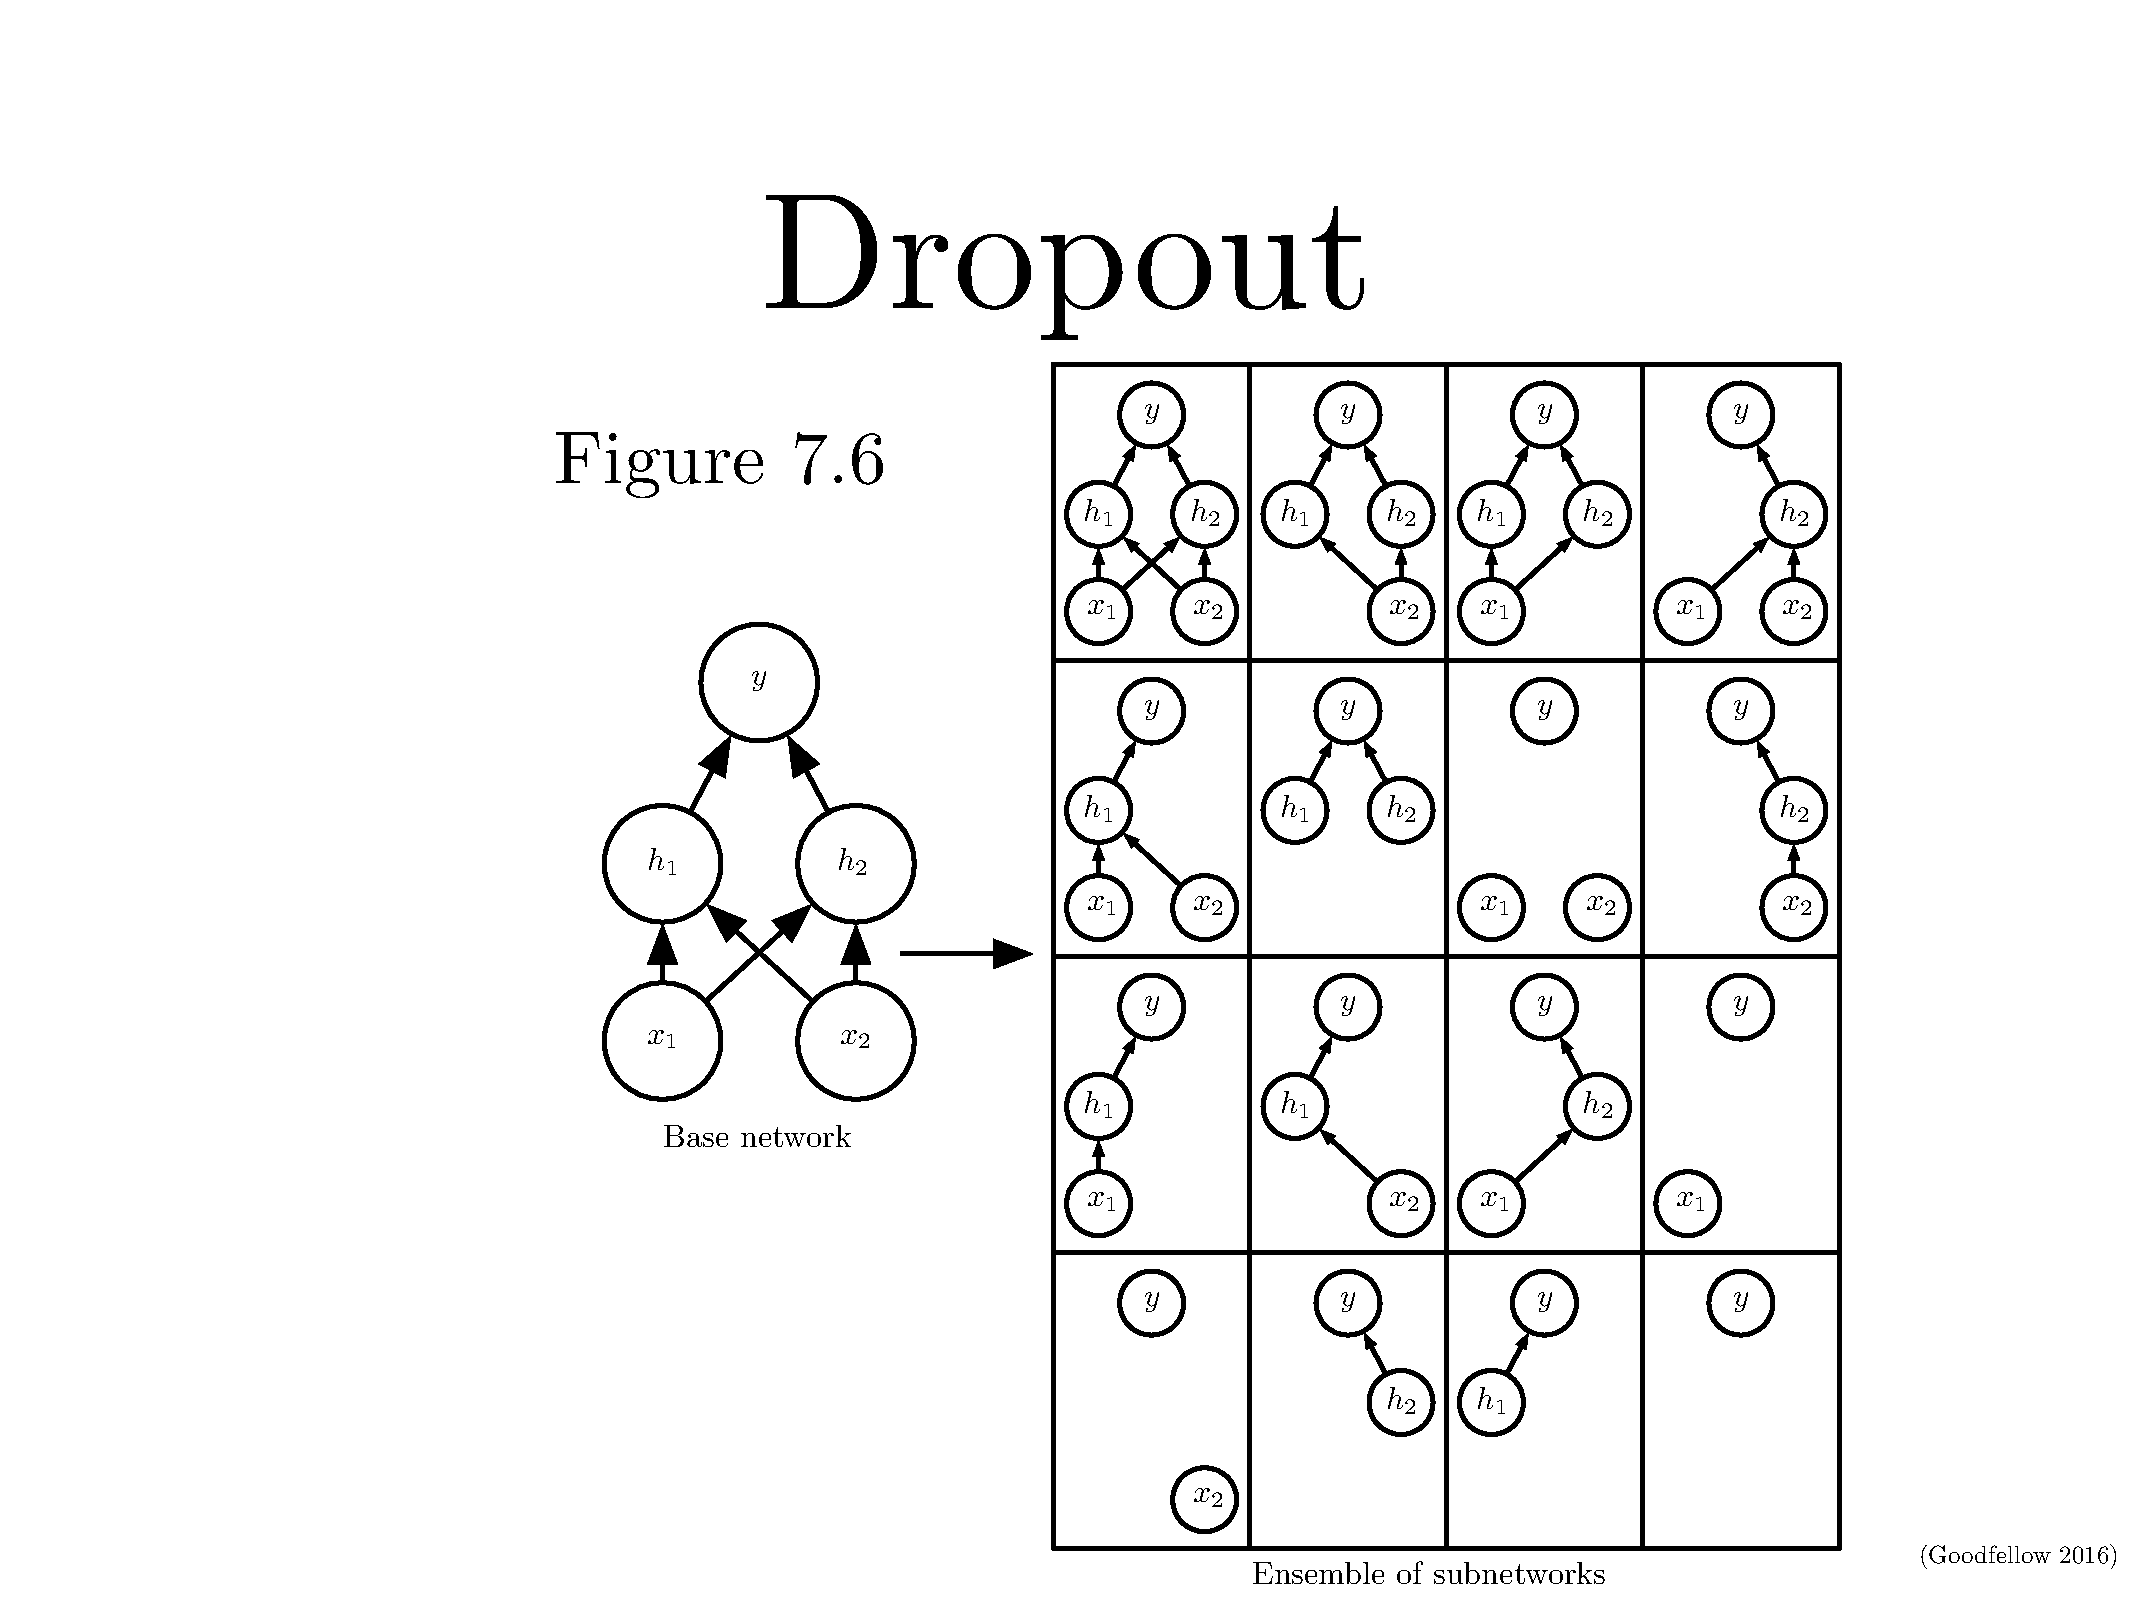
\includegraphics[width=0.75\textwidth]{dropout.pdf}}
  \caption{From Dr. Goodfellow's DL book lecture, Chapter 7.}
\label{fig:dropout}
\end{figure}

\textbf{Dropconnect} (\nurl{http://cs.nyu.edu/~wanli/dropc/}){Li et al 2013}). Generalizes dropout by applying it to edges rather than hidden units. It's not as commonly used as dropout, but it has a more mathematically sound explanation of how its inference procedure mimics ensembles.

\section{Adversarial Training}

(\nurl{https://arxiv.org/abs/1412.6572}{Goodfellow 2014}). Tiny changes in input can result in large differences in output, showing that the learned manifold for a classification category is too sensitive to perturbations in directions that it shouldn't be. Adversarial training forces nets to overcome this.

\end{document}

% LocalWords: Vanhouke
